\section{Introduction}

\subsection{Background}

\subsubsection{Revolve NTNU}

Revolve NTNU is a student organization dedicated to constructing electric formula cars for the international Formula Student competitions. In the course of one year, an electric vehicle (EV) is designed, constructed and tested before entering multiple competitions, facing off against comparable vehicles and teams from other universities from around the world.

\begin{figure}[H]
    \centering
    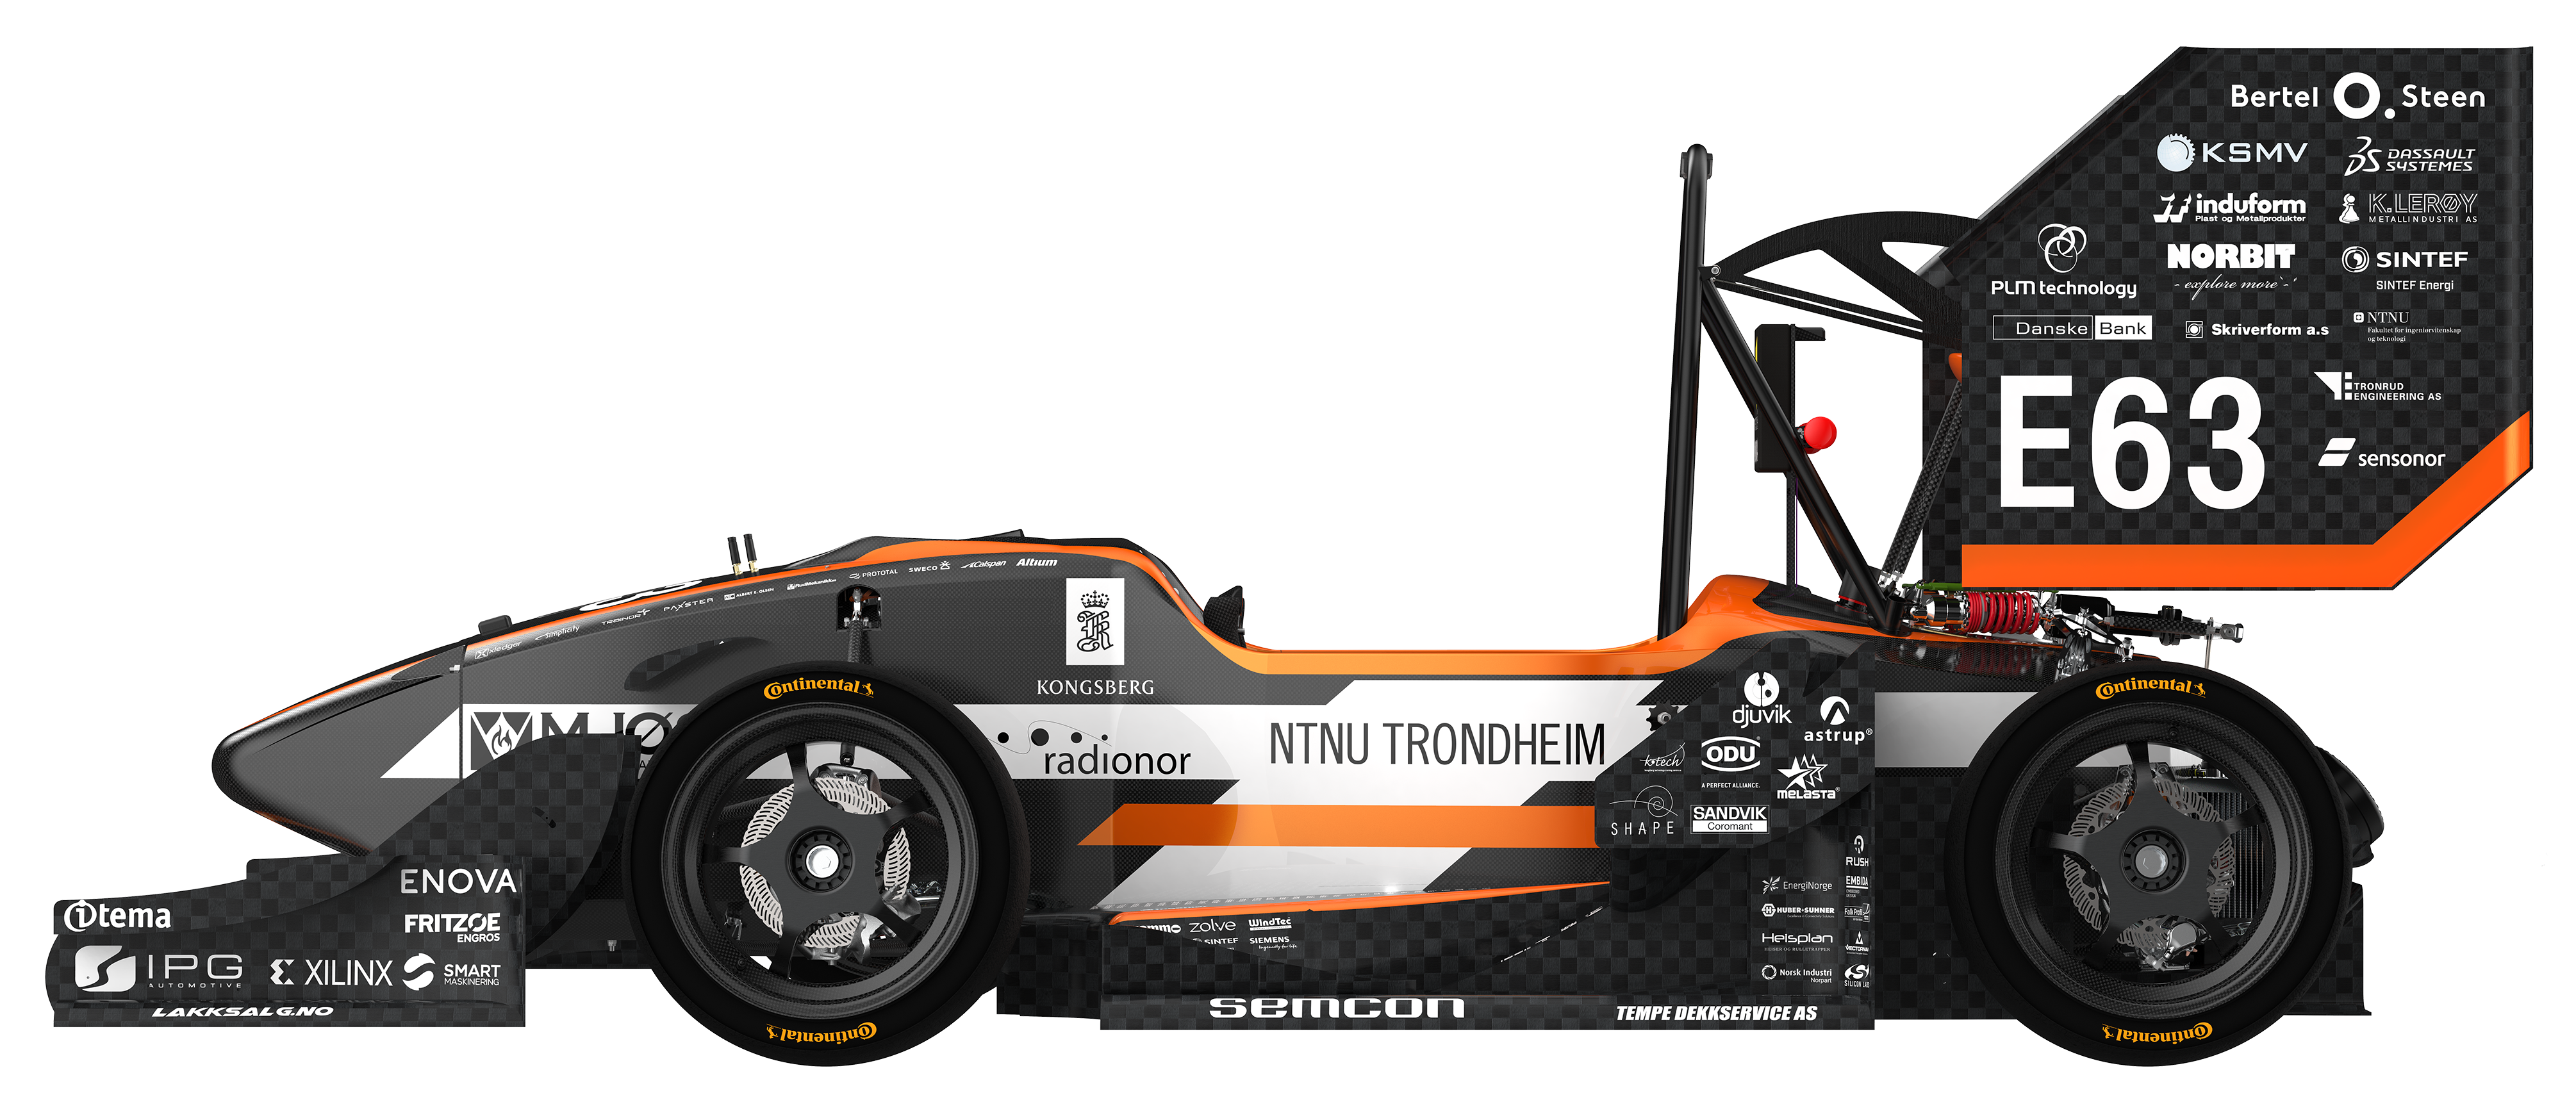
\includegraphics[width=\textwidth]{media/Nova.png}
    \caption{Revolve NTNU 2019's electric vehicle, Nova}
    \label{fig:nova}
\end{figure}

The combination of short development time and a team consisting of mostly new, inexperienced members makes for several interresting problems. This report will focus on a specific embedded system, the vehicle control unit (VCU), and the issues encountered when developing it. As the EV is almost exclusively made from custom parts, the different systems on the car depends heavily on each other. This means that both changes done the VCU will invariably affect the rest of the vehicle and issues with other systems will most certainly affect the VCU. 

To get a clearer picture of necessary changes to the VCU, we start with the system requirements. analyze last year's VCU, VCU19.

\subsubsection{The vehicle control unit}

The vehicle control unit is the central control system of the electric vehicle. That is, it is responsible for inputting sensory data from the vehicle and the driver, and then output fitting data to electric motors connected to each wheel.

In addition, the VCU is to
\begin{itemize}
    \item put the vehicle into Drive-Enable mode when certain criteria are met
    \item perform safety checks on inputted data and take appropriate action if errors are found
    \item interface with the inertial navigation system (INS)
    \item interface with the data logger provided by competition officials, as per EV 4.6 \cite{fsgrules}
\end{itemize}

The team member responsible for the VCU is not responsible for the implementation of the control algorithms that takes vehicle and driver input and outputs motor set points. The control algorithms performs torque vectoring, a technique for intelligently varying the torque on each wheel {\color{red}(reference here)}, increasing the maneuverability of the EV. The VCU is responsible for providing an environment for the control algorithms to run.

Since the vehicle is capable of speeds exceeding 110 kilometres per hour \cite{novaspeed}, the control algorithms cannot use more time than necessary. As the deadlines the VCU has to uphold are critical for the survival of the vehicle and possibly the driver, it is per definition a \emph{hard real-time embedded system}. However, the exact deadline is unknown. The rule of thmub used by members is that the control loop has to run in at no lower than 100 \si{\hertz}. {\color{red}(Should really find some data on this.)}

\subsubsection{Analysis of VCU19}

To fulfill the requirements of the control algortihm, VCU19 was designed around a new processing platform, the Xilinx Zynq-7000. It is a SoC with a dual core ARM Cortex A9 processor and embedded FPGA \cite{zynq}. There were however issues with this implementation. Advanced processing units like the Zynq-7000 are commonly only available in ball grid array (BGA) packages, meaning packages with all pins placed in a grid pattern on the bottom. This makes hand soldering impossible, a reflow method has to be used instead. This makes assembly and debugging harder, a serious concern considering the rapid development methodologies necessary in Revolve NTNU. The high complexity of design also compelled the previous designer to opt for the smallest available package, a 225 pin BGA package. This limits the available peripherals, but was deemed a necessary compromise during the 2019 season.





%\tikzstyle{block}=[draw, thick, minimum size=5mm]

%\begin{figure}[h!]
%    \centering
%    \begin{tikzpicture}[node distance=3cm,auto]
%       %Nodes
%        \node [block] (vcu) {VCU};
%        \node [block] (ins) [right of=vcu] {INS};
%       
%       %Lines
%        \path [<->] (vcu) edge node {RS-232} (ins);
%    \end{tikzpicture}
%    \caption{CAN-FD bus load}
%    \label{fig:canfd}
%\end{figure}

\subsection{Scope}

This report covers the design of VCU20. The main focus of the new design is to reduce the complexity of the system while keeping the performant Zynq-7000 SoC platform. 

%In addition we will take a closer look at the CAN-FD buses connecting the embedded systems on the vehicle.



%\subsection{Interfacing systems}

%The VCU gathers data from other embedded systems on the car. First and foremost we talk about the sonsor broadcasting system (SBS) and the inertial navigation system (INS). 
%\subsubsection{SBS}

%The SBS consists of two equal embedded systems, one placed in the front of the vehicle and one placed in the rear of the vehicle. These boards samples sensor data from and around the wheel and motor assemblies. The SBS's are both connected to the two CAN-FD buses running through the vehicle.

%\subsubsection{INS}

%The INS is an off-the-shelf solution, more precisely a VectorNav VN-300 Rugged. It uses two GPS antennaes, one on the front and one on the main hoop behind the driver, to determine the position, heading, speed and acceleration of the vehicle. The INS has two independent serial interfaces, interface 1 operating on RS-232 voltage levels, and interface 2 operating on TTL voltage levels. The only difference between the two interfaces in terms of functionality is that firmware update of the INS is available through interface 1 only. 

%This, in addition to the higher voltage used on interface 1 making it more resistant to noise, is the reason VCU19 communicated with the INS over interface 1. Note that this requires a TTL to RS-232 level shifter circuit on the VCU.

%\subsubsection{Inverters}

%The inverters converts the DC voltage from the high voltage batteries to a three-phase AC which can be used to drive the electric motors. This is by far the most complex embedded system on the vehicle. It consists of two controller cards, each controlling two inverter power cards. This makes for a total of four motor inverters, one for each motor. The inverter control cards are connected to the two CAN-FD buses, accepting messages containing \emph{set points} for the inverters, meaning how fast each motor shall turn.

%\subsubsection{Telemetry}

%The telemetry system on the vehicle is a long range radio transciever that allows for communication and monitoring of the car from a base station. The radio system is a RadioNor CRE2-144-LW which utilises phase-shift arrays to transmit signals reliably over long distances. The radio interfaces with the vehicle through an Ethernet port, receiving and transmitting UDP packages. In 2019, no other embedded system on the car used Ethernet, and a Respberry Pi 3 B+ was connected to the CAN-FD buses with two PCAN-FD USB dongles so that the embedded systems could interface with the telemetry.

%\subsubsection{Torque vectoring}

%Torque vectoring is the software system that takes the current state of the car and translates this to a desired torque on each of the four motors. It allows for better vehicle handling, especially in turns. It is a software system which should run on the VCU, but the code itself is developed and maintained by another team member. It is therefore crucial that the VCU is capable of running the TV regulation loop at a certain frequency and can supply the required resources (memory and storage). Research shows that the TV control loop has to run at 100Hz minimum to be effective.
 


